\documentclass{article}
\usepackage{amsmath}
\usepackage{fancyhdr}
\usepackage{amsthm}
\usepackage{amsfonts}
\usepackage{cite}
\usepackage{float}
\usepackage{scrextend}
\usepackage{hyperref}
\usepackage{caption}
\usepackage{subcaption}
\theoremstyle{definition}
\newtheorem{theorem}{Theorem}
\newtheorem{definition}{Definition}
\newtheorem{goal}{Goal}
\newenvironment{sketchproof}{%
  \renewcommand{\proofname}{Sketch of Proof}\proof}{\endproof}
  
\setlength{\parindent}{0pt}

\usepackage{Sweave}
\begin{document}
\input{LoanPricing-concordance}

\section{Introduction}



\section{Mathematical preliminaries and definitions of loans}
Before diving in on pricing theory, it is useful to consider the definition and characterization of loans.  Loans involve the providing of an asset from party A (the lender) to party B (the borrower).  In return, party B pays party A over a (often predefined) set of times.  The terms of the loan typically require the sum of party B's payments to be greater than the original amount of money transferred to party B.  The excess of money that B pays A is called ``interest''.  The annualized percentage of interest relative to the original transfer is called the ``interest rate''.  

\subsection{Mathematical formulation}
Put mathematically, a loan involves an exchange of money \(P_t\) from the lender to the borrower at time \(t\).  The borrower then cumulatively pays the lender \(\int_t ^ \infty c_s ds\) for the original amount \(P_t\).  The value \(P_s\) is the par or ``book'' value of the loan.  It represents the amount of the original transfer that is owed at time \(s \in (t, T)\).
\\
\\
Typically, there is some point \(T\) which satisfies \(c_s=0\, \forall\, T<s<\infty\); that is \(T= \sup\{c_s>0 | s>=t\} \).  At this point \(T\) the value \(P_T\) is zero.  The loan is considered to be closed and neither party is beholding to the other.  
\\
\\
Another common feature of loans is that the cash flows tend to be discrete.  This enables us to use a summation instead of an integral for the cash flows.  More importantly, it allows us to model the cash flows as a series of separate (though potentially dependent) assets.  Unless specified otherwise, we will treat each cash flow independently in this book.  This enables us to define a loan as a contract in which \(P_t\) is transferred from the lender to the borrower at time \(t\) and in which the borrower promises to transfer \(c_T\) at time \(T\). For such a loan it is reasonable (though not required) to have \(c_T>P_t\).  Note that for a loan with a series of cash flows the reverse is typically true (\(c_T<P_t\)).  
\\
\\
The purpose of considering a single transfer is that it makes the exposition and mathematical derivations more clear.  It does so without losing too much generality. 

\subsubsection{A digression into yield and interest rate}

Interest rates and yields are very similar but also quite distinct.  The interest rate is the contractual rate which determines the size of the cash flows.  For example, in a simple coupon bond with \(P_t=1\) and interest rate \(5\%\) with annual cash flows for \(4\) years, the bond will be exchanged at time \(t\) for \(1\) dollar.  At years \(t+1,\,t+2, \,t+3\) the bond will pay \(5\) cents.  In the fourth year the bond will pay \(1.05\) dollars.  The interest rate stays constant over the life of this loan and is part of the original contract.  The yield is a metric used to measure the rough return of the bond.  For example, if the bond immediately after issuance started trading at \(0.98\) dollars, the yield would be higher than \(5\%\) since the coupon of \(5\) cents is being paid on a price of \(.98\) instead of on a dollar.  
\\
\\
This is even easer to see for a zero-coupon bond.  A zero coupon bond is one that pays back (without loss of generality) one dollar at time \(T\) with no intermediate payments.  An interest rate of \(5\%\) on a zero coupon bond with maturity in one year has \(P_t=e^{-.05}\approx .951\).  If this bond instantaneously started trading at \(.96\), the yield would be approximately \(4.1\%\).  
\\
\\
The difference between an initial (contractual) price or value and a value after origination will be a common theme.  
\\
\\
While interest rates and yields are convenient metrics to compare various investments and loans, we find that they confuse the narrative.  Given a value or price of a loan it is trivial to compute yields or interest rates.  This book focuses on finding the appropriate price of the loan and considers interest rates when discounting.

\subsection{Risks}
Loans introduce risk to the lender.  There are two primary risks: interest rate risk and credit risk.  Interest rate risk is the risk that alternative investments may be more attractive at some point \(\tau>t\).  However, there is often no good way to ``undo'' the loan and take advantage of alternative investments.  Credit risk is the risk that the borrower does not pay the agreed upon cash flow; that is, the borrower defaults.  
\\
\\
There are some ways to remediate or immunize these risk.  Interest rate risk can be reduced in several ways.  First, there may be conditions in the loan that allow the lender to ``call'' the loan and require immediate repayment.  These are typically rare.  Second, the loan may have a variable rate.  As market interest rates move, the payment \(c_s\) will change to accommodate.  While this helps reduce interest rate risk, it may increase credit risk since the borrower's ability to service debt may be impaired.   Third, the lender may purchase a swap to offset the interest rate risk.  Purchasing a swap brings another party to the table and may increase credit (or counterparty) risk.  
\\
\\
Credit risk can be reduced by requiring that the borrower post collateral.  In the event of default, the lender will receive the collateral.  There is still credit risk involved with securitized loans.  The collateral could depreciate to be lower than the value of the future contractual cash flows; leading to a loss.  The physical act of taking possession of the collateral may require time and resources.  
\subsubsection{Modeling Risk}
The economic definition of risk is uncertainty.  The mathematical model of uncertainty is probability.  To reflect the loan's credit risk, the cash flows from the loan can be written as 

\begin{equation} \label{riskyCashFlows} 
\int_t ^ T c_s \mathbb{I}_{\tau>s} ds+\mathbb{I}_{\tau<T} k_\tau \end{equation}
Where \(\mathbb{I}\) is the indicator function, \(\tau\) is the (random) time of default, and \(k\) is the cash flow generated from sale of collateral.  
\\
\\
In our simpler model of a single cash flow, the equation can be simplified as follows:

\begin{equation} \label{simpleRiskyCashFlows}
c_T \mathbb{I}_{\tau>T}+\mathbb{I}_{\tau<T} k_\tau
\end{equation}


\subsubsection{Risk free asset} \label{rfasset}

It is often convenient to assume the existence of a risk free asset \(M_t\).  By definition, the risk free asset returns
\[\frac{dM}{dt}=r_{f, t} M\]
Solving this ODE yields
\[M_T=M_t e^{\int_t ^T r_{f, s} ds}\]

Note that \(r_{f, t}\) is allowed to be stochastic.  Default free bonds can be considered derivative securities of this risk free asset.  The only risk in default free bonds (eg, Treasuries) is interest rate risk.  A common asset in this book will be a zero coupon bond which has a single cash flow \(c_T\).  These assets are denoted \(B(t, T)\). 

\subsection{Value through time}
\label{valOfCashFlows}
The stream of cash flows defined in \ref{riskyCashFlows} has some value at every point \(s \in (t, T)\).  This value is denoted \(V_s\).  While we have not yet developed the toolkit in this book to approach finding the ``appropriate'' value \(V_s\), intuitively it should depend, in some sense, on the cash flows defined in \ref{riskyCashFlows}.  Put mathematically, 
\[V_s=g\left(   \int_s ^ T c_u \mathbb{I}_{\tau>u} du+\mathbb{I}_{s<\tau<T} k_\tau  \right) \]

The function \(g\) may depend on other variables aside from the cashflows.  The value does not depend on cash flows that have already been paid, which is reflected in the updated lower bound of the integral.  If default has occurred before \(s\) (and collateral has been sold) \(V_s\) should be zero.
\\
\\
Note that the simpler model defined in Equation \ref{simpleRiskyCashFlows} cannot be simply added up to retrieve the actual price of a loan.  Let the following be the price or value of a single cash flow:
\[
v_j= g\left(c_{t_j} \mathbb{I}_{\tau>t_j}+\mathbb{I}_{\tau<t_j} k_\tau\right)
\]

Unless \(g\) is linear, there is no obvious method for computing \(V_s\) as a function of the \(v_j\).


\subsection{Modeling considerations: the loan market}
\label{loanMarket}
There are two markets for loans: the primary market where lenders and borrowers agree on terms for exchanging cash flows, and a secondary market where the promised cash flows can be exchanged.  For example, mortgage lenders will agree to terms with home buyers.  Mortgage lenders will then typically sell these loans to Fannie Mae.  Fannie Mae packages these loans and sells them to hedge funds, mutual funds, and other institutional investors.  
\\
\\
A secondary market does not always exist for loans which makes loan pricing both challenging and potentially rewarding. Most asset pricing literature considers that there is a market with prices for most if not all instruments.  This is the fundamental assumption for the models summarized in Section \ref{assetPricing}.  Indeed, practitioners in capital and equity markets frequently mark their models to market.  They assume a certain model for the market and then use market prices to calibrate the model.  
\\
\\
However, in general the value \(V_s\) from Section \ref{valOfCashFlows} is not a price that is viewable in the market.  This can have benefits to the lender.  If the lender believes that a borrower has better credit worthiness than the (primary or secondary) market, the lender can originate a loan at better than cost.  However, if the price is viewable in the market, the lender can make the loan ``available for sale'' (AFS).  This requires the loan to be marked to market.  Even if the lender believes the loan is higher quality, the loan will be booked as if it is lower quality with the requisite capital charge.  If the lender is right, the loan will still provide superior cash flows than expected.  This higher quality won't be reflected in the balance sheet at the time of origination. 
\\
\\
If the loan is not available for sale then the loan is booked at ``par''; that is, the value of the asset is the amount lent \(P_t\).  A simple decision for whether to originate a loan could then be 

\begin{equation}
\left\{
\begin{array}{ll}
\text{originate loan if} & V_t \geq P_t\\
\text{do not originate otherwise} 
\end{array} \right.
\end{equation}

This decision is naive.  First, a loan is required to have additional reserves for expected losses under accounting rules (SEE LATER SECTION).  Second, a loan requires capital to withstand losses that are greater than expected.  Again, this will defined more rigorously in a later section.  

\subsection{Goal of this book}

The goal of this book is introduce methods for finding the ``appropriate'' price of a loan.  Section \ref{valOfCashFlows} introduces the notion that the stream of cash flows \ref{riskyCashFlows} has some value \(V_s\) at every point in time \(s\).  The lender and the borrower agree at origination time \(t\) on the structure of the cash flows.  The implicit goal in section \ref{valOfCashFlows} is that \emph{given} a series of cash flows there is some method of computing the current value of those cash flows.  The goal for the lender at time \(t\) is to find a set of cash flows such that the value \(V_t\) is maximized.  This goal is summarized as follows:

\begin{goal}[Lender's problem] \label{lender1}
	\[\max_{c_s} V_t\]
	
\end{goal}

There are three considerations not explicitly shown in this equation which makes the goal ill-posed.  First and most importantly, the borrower is able to decline the offer.  As \(c_s\) increases, the probability of the borrower declining the offer increases.  The second consideration is that as \(c_s\) increases there is an increase in the probability that \(\tau<T\).  The borrower will have less ability to service the cash flow and is more likely to default.  The third consideration is related to both the first two considerations and to the fact that the borrower has asymmetric information about his or her ability to repay the loan: as \(c_s\) increases, any borrower that does accept the offer is more likely to be a poorer quality customer.  The fact that the borrower chose a higher \(c_s\) indicates that there is little appetite for the borrower's risk in the market.  At a very high level of \(c_s\), the borrower is likely going to take the cash and run with no intention of repayment.  This is especially the case for subprime retail portfolios.  
\\
\\
These three considerations can be captured by considering the market cash flows \(c_{m, s}\).  However, as any loan officer will say, Goal \ref{lender1} is incorrectly stated.  Rather, in a competitive (primary) market, the cash flows \(c_s\) are ``fixed'' for a given level of ``widely available'' measures of risk (say, a level of debt service coverage).  Instead of choosing the cash flow to maximize the value functions from Section \ref{valOfCashFlows}, the goal is to find areas where the lender can more accurately assess the probability that \(\tau<T\) and thus undercut the (primary) market.  
\\
\\
There are several mathematical methods for considering this phenomenon.  Perhaps the simplest is to model the ``market'' belief that the time to default random variable is \(\tau_m\) and the lender's belief is that the time to default random variable is \(\tau\).  The lender's problem then becomes the following:


\begin{goal}[Lender's problem revisited] \label{lender2}
	\[
	\left\{
	\begin{array}{ll}
	\text{originate loan if} & V_t\geq V_{t, m}\\
	\text{do not originate otherwise} 
	\end{array} \right.
	\]
	
\end{goal}

Where \(V_{t, m}\) is the market's valuation of the expected future cash flows.  Goal \ref{lender2} has the benefit of being most similar to how lenders typically run their business.  Unfortunately, goal \ref{lender2} is not academically appealing.  As seen in Section \ref{assetPricing}, models for asset pricing typically assume that the market is correct.  Hence the formulation of goal \ref{lender2} is nonsensical.  The reason that goal \ref{lender2} makes some sense is the following:


\begin{enumerate}
	\item The loan market tends to be illiquid; that is, the value \(V_t\) is not a market price but a subjective valuation of the future cash flows.
	\item Loans that are securitized and made available on the market tend to have high level risk characteristics but may have idiosyncrasies that are only visible to the lender; that is, there is asynchronous information between the lender and the market.  
	\item The market does not always trust in the competency of lenders.  This can be seen by market prices of securitizations from new lenders.  These securitizations may look the same as from established lenders, but they will typically trade at a lower value simply because there is not as much trust that the lenders have the ability to originate quality loans.  
	
\end{enumerate}

Other shortcomings with goal \ref{lender2} is that it assumes the capital structure and loan mix is identical between the market and the lender.  

\section{Introduction to Asset Pricing} \label{assetPricing}

There are three primary academic approaches to asset pricing.  The original approach is founded in utility theory.  This approach is theoretically rigorous but lacks precision.  It is best described as a phenomenological model of asset pricing but is not intended to provide a framework for precisely pricing assets.  However, the other two pricing approaches are consistent with this original approach and owe much to utility theory.  The second approach is the theory Capital Asset Pricing Model approach pioneered by Markowitz, Sharpe, and others.  Markowitz developed a theory around choosing optimal portfolios assuming either quadratic preferences or Gaussian asset returns.  Sharpe created a way to estimate what the expected return of an asset should be based off the correlation with the rest of the market.  This approach is more precise than utility theory but is prone to model error.  It is not easy to generalize the approach.  Again, the approach is primarily a good mental model for asset pricing.  The third approach is the replicating portfolio argument pioneered by Black and Scholes.  This technique is primarily applicable to derivative securities where the price can be determined by other assets.  The approach has proved very precise and rigorous.  It has also proven extensible and general.  
\\
\\
This section is devoted to more detailed descriptions of these three approaches.  The section motivates various ways of thinking about loan pricing.

\subsection{Utility theory}
Utility theory states than a given individual (homo economicus) seeks to maximize a function \(U\) that satisfies the ``usual'' conditions:
\begin{enumerate}
\item \(U'(x)>0\)
\item \(U''(x)<0\)
\end{enumerate}

In general, utility functions need not be continuous and don't require derivatives to be defined.  Indeed, all that is required for our discussion is that the utility function is concave.  However, since exact results are not required from this approach for our purposes, the useful mental picture is to assume continuity and differentiability.
\\
\\
The above conditions imply non-satiability and risk-aversion.  Risk-aversion is the more important aspect from an asset pricing perspective.  By Jenson's inequality, 
\[\mathbb{E}[\phi(X)]<=\phi(\mathbb{E}[X])\]
for concave \(\phi\).  For a risky asset \(Y\), the value placed on the asset by an individual with utility function \(U\) is \(\mathbb{E}[U(Y)]\).  This is less than the utility gained from the expected value of the asset.  The return required by the individual for the asset \(Y\) is higher than a return for a degenerate (non-risky) asset \(Z\).   
\\
\\
Applying this theory to the cash flow equation \ref{simpleRiskyCashFlows} the utility gained is

\[\mathbb{E}\left[U\left( c_T \mathbb{I}_{\tau>T}+\mathbb{I}_{\tau<T} k_\tau \right) \right]\]

If both the utility function and the distribution of \(\tau\) is known, in theory we could create the indifference curve between the utility of holding the money (or investing in a risk-free asset) and the utility of lending out the money and receiving the cash flows.  However, the utility function is only applicable to a ``representive agent'' and is very difficult to estimate in practice.  Additionally, in reality there is a large set of investments.  It is impracticable to optimize over the entire investment set.  Markowtiz solved this problem under a certain set of assumptions with modern portfolio theory.  

\subsection{Modern Portfolio Theory and CAPM}
Under the assumption that asset returns are Gaussian, Markowitz formulated an optimization problem specifying the amount to invest in every asset in the market.  The theory reduces the problem of utility optimization to one that explores the tradeoff between variance and expected returns.  For a given level of variance (risk-tolerance), the goal of the problem is to maximize the return.  The theory formalizes and makes a precise recommendation around the notion of asset diversification.  However, the theory treats expected returns and variances as fixed and known constants.  The price of the assets are not modeled; rather if every market participant followed the mean-variance recommendations there would be a market-based price for every asset based on the prevailing level of risk-tolerance.  
\\
\\
Sharpe used the theory to compute the expected return for a given stock.  To gain intuition for Sharpe's theory, consider a world in which the following is true:
\begin{enumerate}
\item There exists an infinite number of assets
\item The returns of these assets are independent (uncorrelated)
\end{enumerate}

A portfolio that contains these assets would have zero variance.  A portfolio that has no risk must return the risk free rate in equilibrium.  Using this intuition, any risky asset should return excess of the risk free rate only through its correlation with the rest of the market.  This leads to the celebrated CAPM formula 
\[\mathbb{E}[r_{i, t, T}]=r_{f, t, T}+\beta_i \left(\mathbb{E}[r_{m, t, T}]-r_{f, t, T}\right)\]
The \(\beta\) is the effect that the market has on the expected return on the asset \(i\).  A \(\beta\) of zero corresponds with an expected return of \(r_f\), or the risk free rate.
\\
\\
While loans do not have Gaussian returns, the theory still has application for loan pricing.  The primary relevance of CAPM on loan pricing is the concept of diversification and the dependence of the price of an asset on the existence of other assets.  In a large portfolio of uncorrelated loans and in an efficient market, the interest rate should only compensate for the expected loss of the loan.  
\\
\\
Let the \emph{loss distribution} of a portfolio of \(n\) loans be defined as follows:

\begin{equation}
\mathbb{P}(L<l)
\end{equation}

Where \(L=\sum_i X_i \) and \(X_i\) is the random variable describing the risky cash flows of loan \(i\).  As proven in Vasicek (1989), if \(\mathbb{E}[X_iX_j]-\mathbb{E}[X_i]\mathbb{E}[X_j]=0\,\forall\,i,\,j\) then \( \lim_{n \to \infty}\mathbb{V}[L] \to 0\).  By the linearity of expectations, the expected gain for \(L\) is simply \(\sum_i \mathbb{E}[X_i]\).  In equilibrium, this expected gain must equal the risk free rate since the portfolio has no risk.  If we further assume that the loans are homogeneous, we can also exactly find the ``correct'' price for each loan as follows: choose \(c_T\) such that

\[
\left\{c_T \,|\, \mathbb{E}\left[ c_T \mathbb{I}_{\tau>T}+\mathbb{I}_{\tau<T} k_\tau \right]=B(t, T)\right\}
\]

\subsection{Black Scholes and Risk Neutral pricing}

In 1973 Black and Scholes published their seminal paper on derivative pricing.  They showed that, under some assumptions, a certain class of derivative securities are ``redundant'' in the market; that is they can be replicated by trading in two simple assets.  This breakthrough has three primary advantages over CAPM and modern portfolio theory: it is extremely precise, does not depend on equilibrium theory (ie, it only requires the prices of a small subset of assets, and does not require estimating the expected return on an asset.  
\\
\\
Generalizations of this work show that in a complete market, the price of any derivative security can be written as an expectation.  The expectation is not under the ``real world'' probability measure but instead the ``risk-neutral'' probability measure.  
\subsubsection{Example of Risk Neutral pricing} \label{RNExample}
There have been many attempts at explaining ``risk-neutral'' pricing intuitively.  In the author's opinion, there is no simple explanation to do risk-neutral pricing justice.  In essence it is a computational trick which allows us to price using expectations.  For example, consider a simple two-state model with a stock, a risk free bond, and a call option on the stock.  The stock is currently at value \(S_0\).  The stock can be at \(S_u>S_0\) or \(S_d<S_0\) in period \(1\).  The bond is currently at value \(M\).  The value is at \(M\) in one period.  The option pays \(C_u=S_u-K\) if the stock goes up or \(C_d=0\) is the stock goes down.  
\\
\\
Consider the following strategy: construct a portfolio \(X_0\) at time \(0\) comprised of \(\Delta\) stock and \(\Gamma\) bonds.  The goal is to find \(\Delta\) and \(\Gamma\) such that at time \(1\), the final value of the portfolio is equal to the option payoff.  The problem can be solved using a simple matrix approach:

\[
\begin{bmatrix}
	M & S_u \\
	M & S_d 
\end{bmatrix}
\begin{bmatrix}
\Gamma \\
\Delta 
\end{bmatrix}
=
\begin{bmatrix}
S_u-k \\
0.0
\end{bmatrix}
\]

Using standard matrix algebra and substituting back into the formula for \(X_0\), 

\[X_0=\frac{S_0-S_d}{S_u-S_d}\left(S_u-k\right)\]

Note that \(0<\frac{S_0-S_d}{S_u-S_d}<1\) and can be interpreted as a probability.  Indeed, 

\[X_0=\tilde{p}C_u+(1-\tilde{p})C_d =\mathbb{\tilde{E}}[C]\]

Where \(\tilde{p}=\frac{S_0-S_d}{S_u-S_d}<1\).  Note that this is simply a convenient representation and has very little to do with actual probabilities of stock price movement.  The only relevance that the actual probabilities have is on the initial stock price \(S_0\).  If the actual probability of an ``up'' movement is very small then the initial stock price will likely be much closer to \(S_d\).  This will have a corresponding impact on the risk-neutral probability of an up move.  
\\
\\
By no arbitrage, the price of \(C\) at time \(0\) must be equal to \(X_0\).  Hence we have found the ``correct'' price for \(C\).  
\subsubsection{Risk-neutral pricing without a replicating portfolio}

The argument from Example \ref{RNExample} is predicated on the ability to replicate the option price with a bond and the stock.  Can a similar representation of an asset hold in the case for assets that cannot be replicated?  There seems to be some hand-wringing about this in the literature.  However, we rely on (F. Delbaen and W. Schachermayer 1998 https://people.math.ethz.ch/~delbaen/ftp/preprints/NLB.pdf) to prove the following general theorem:

\begin{theorem}[First Fundamental Theorem of Asset Pricing] \label{FFTAP}
	For a multidimensional semimartingale \(S_t\) (representing the ``market''), the following are equivalent:
	\begin{enumerate}
		\item There exists a probability measure under which \(S_t\) is a martingale
		\item The market does not admit \emph{free lunch with vanishing risk}
	\end{enumerate}
\end{theorem}

The notion of free lunch with vanishing risk essentially replaces the strong notion of no-arbitrage with the weaker notion of \(\mathcal{L}_2\) convergence.  For our purposes, the weaker notion is sufficient. 
\\
\\
Theorem \ref{FFTAP} does not provide any hints at how to price an instrument.  Indeed, if an asset cannot be replicated then there are theoretically infinite prices for the asset.  However, we follow the convention of using a measure induced by the risk neutral asset.

\subsubsection{Asset pricing without replication}

The price of an asset in this book is assumed to have the following representation:

\[\frac{X_t}{M_t}=\mathbb{\tilde{E}}\left[\frac{h(S_T)}{M_T}|\mathcal{F}_t\right]\]
Where \(S_T\) is a process that \(X_s\) depends on (eg, the stock in Example \ref{RNExample}) and \(M_t\) is the risk free asset from Section \ref{rfasset}.  Note that this representation implies that \(\frac{X_s}{M_s}\) is a martingale.  

\subsubsection{Zero-coupon bond}
The price of a zero-coupon bond with no credit risk is the following:

\[B(t, T)=\mathbb{\tilde{E}}\left[\frac{M_t}{M_T}|\mathcal{F}_t\right]\]
\[=\mathbb{\tilde{E}}\left[e^{-\int_t ^ T r_s ds}|\mathcal{F}_t\right]\]

There are a variety of models for the instantaneous interest rate for which there are closed form solutions for \(B(t, T)\).  

\subsubsection{Basic loan with potential for default}
Consider a simple model with the risk-free asset having no return (risk free rate of zero). There is a loan that has a \(3\%\) probability of default before maturing in a year.  There is no recovery at default.  The expected value of the loan is \(0.97\).  However, the price of the loan will be less than \(0.97\) to compensate for the risk of the loan.  The risk-neutral probability of default is very simple to back out of the price: \(\hat{p}=1-S_t\) where \(\hat{p}\) is the risk-neutral probability of default and \(S_t\) is the price of the loan.  However, as mentioned in \ref{loanMarket}, there often is not a secondary market for loans.  
\\
\\
The amount of capital that a financial institution holds acts as a shield or buffer against loan losses.  This capital tends to be expensive (most estimates place the required return on capital in the 12\% to 20\% range) and must be taken into account when considering the price of a loan.  Indeed, in an ``equilibrium'' world, the ``risk-neutral'' return on a loan will exactly equal the expected default rate plus the required capital costs.
\section{Partial Equilibrium Model for Loan Pricing}

And now for something completely different!  So far I have have talked about general equilibrium and and risk-neutral pricing.  I now pivot to a model of partial equilibrium with a very specific (but common!) market in retail banking.  

\subsection{Assumptions}
I assume a market with default rates distributed as a Beta distribution, with parameters \(\alpha,\,\beta\).  There are two firms in this market, each providing funds to borrowers.  I assume that there are no operational costs and that each firm requires compensation only for capital charges and expected losses.  To further simplify the analysis, the capital charges are inputs into the model; making this model a partial equilibrium model.  The capital charges are also fixed for every loan made.  This assumption may be appropriate for markets where the loans have fixed regulatory capital charges (eg, home equity loans have a fixed 100\% regulatory capital charge).  Both firms choose the interest rates charged in order to maximize profits.  Note that none of these assumptions is particularly prohibitive and are made to ease the analysis.  Endogenous capital charges are extremely difficult to accurately model and most firms estimate capital charges from internal assessment of credit quality and not from a general-equilibrium model.  

\subsection{Neither firm differentiates, both firms are identical}

In the first scenario, I assume that both firms know \(\alpha\) and \(\beta\) but are unable to determine where the borrower falls in the distribution.  In this case, both firms will require borrowers to at least compensate for the population expected loss rate and any capital charges.  This minimum loss rate is the rate such that the firm is exactly compensated for the expected loss.  Mathematically, 
\[(1+r_{min})\left(1-\mathbb{E}[L]\right)=1+c\]
Where \(r_{min}\) is the minimum rate that the firms will accept and \(c\) is the capital charge.  
Rearranging, 
\[r_{min}=\frac{1+c}{1-\mathbb{E}[L]}-1=\frac{(\alpha+\beta)c+\alpha}{\beta}\]

With both firms identical, this forms a Bertrand Duapoly and the equilibrium rate is simply the minimum rate \(r_{eq}=r_{min}\) at which each firm makes 4\% return on capital.

\subsection{One firm differentiates}

Now I assume that one of the firms have complete knowledge of the risk of a borrower while the other firm still only has knowledge of \(\alpha\) and \(\beta\).   As expected, this will cause the non-differentiated firm to be adversely selected.  To demonstrate this, I delve into the mathematics and demonstrate the results with some plots.

The ``break even'' price for the differentiating firm is now described as follows:

\[\frac{1+c}{1-x}-1\]

For any default probability \(x\).  The strategy for the differentiating firm is now clear: for all loans that are ``overpriced'' by the previously defined \(r_{min}\), charge \(r_{min}\), and then let the non-differentiating firm take the rest.  The profit rate for the differentiating firm is thus:

\[\frac{1}{F(q_{ex};\alpha,\beta)}\int_0^{q_{ex}} \left((1+r_{min})(1-x)-1\right) f(x;\alpha,\beta)dx\]

Where \(f(x;\alpha,\beta)=x^{\alpha-1}(1-x)^{\beta-1} /B(\alpha, \beta)\) is the density function of the Beta distribution, \(F\) is the cumulative distribution function for the Beta distribution, and \(q_{ex}\) is the fraction of loans that are less than the expectation of the Beta distribution.  Indeed, this can be generalized for any rate that the non-differentiating firm chooses:

\[\frac{1}{F(q;\alpha,\beta)}\int_0^q \left((1+r)(1-x)-1\right) f(x;\alpha,\beta)dx\]

Where \(q = \sup_y \left\{ (1+r)(1-y) \geq 1+c\right\} \). 

Solving for \(q\), 

\[q=\frac{r-c}{1+r}\]

The market share for the differentiating firm is simply \(F(q)\), where \(F\) is the cumulative distribution function of the Beta distribution.

\subsubsection{Profit for each firm}
Identifying the differentiating firm by the subscript \(1\) and the non-differentiating firm by the subscript \(2\), the profit rate for each firm is as follows:
\begin{equation}
\pi_1(r)=\frac{1}{F\left(\frac{r-c}{1+r};\alpha,\beta\right)}\int_0^{\frac{r-c}{1+r}} \left((1+r)(1-x)-1\right) f(x;\alpha,\beta)dx
\end{equation}

\begin{equation}
\pi_2(r)=\frac{1}{1-F\left(\frac{r-c}{1+r};\alpha,\beta\right)}\int_{\frac{r-c}{1+r}} ^ 1 \left((1+r)(1-x)-1\right) f(x;\alpha,\beta)dx
\end{equation}

By standard properties of the Beta distribution, these equations can be simplified:
\begin{equation}
\pi_1(r)=\frac{(1+r)\beta}{\alpha+\beta}\frac{F\left(\frac{r-c}{1+r};\alpha,\beta+1\right)}{F\left(\frac{r-c}{1+r};\alpha,\beta\right)}-1
\end{equation}

\begin{equation}
\pi_2(r)=\frac{(1+r)\beta}{\alpha+\beta}\frac{1-F\left(\frac{r-c}{1+r};\alpha,\beta+1\right)}{1-F\left(\frac{r-c}{1+r};\alpha,\beta\right)}-1
\end{equation}



Since the differentiating firm will choose the rate to charge based off the choice of rate by the non-differentiating firm, it is interesting to view charts of the profit and market share for each firm for varying levels of \(r\).

In the charts below, \(\alpha=2\), \(\beta=48\), required return for capital is 4\%, yielding an equilibrium rate of \(1/12 \approx 0.0833\).



\begin{figure}
\centering
\begin{subfigure}{.5\textwidth}
  \centering
 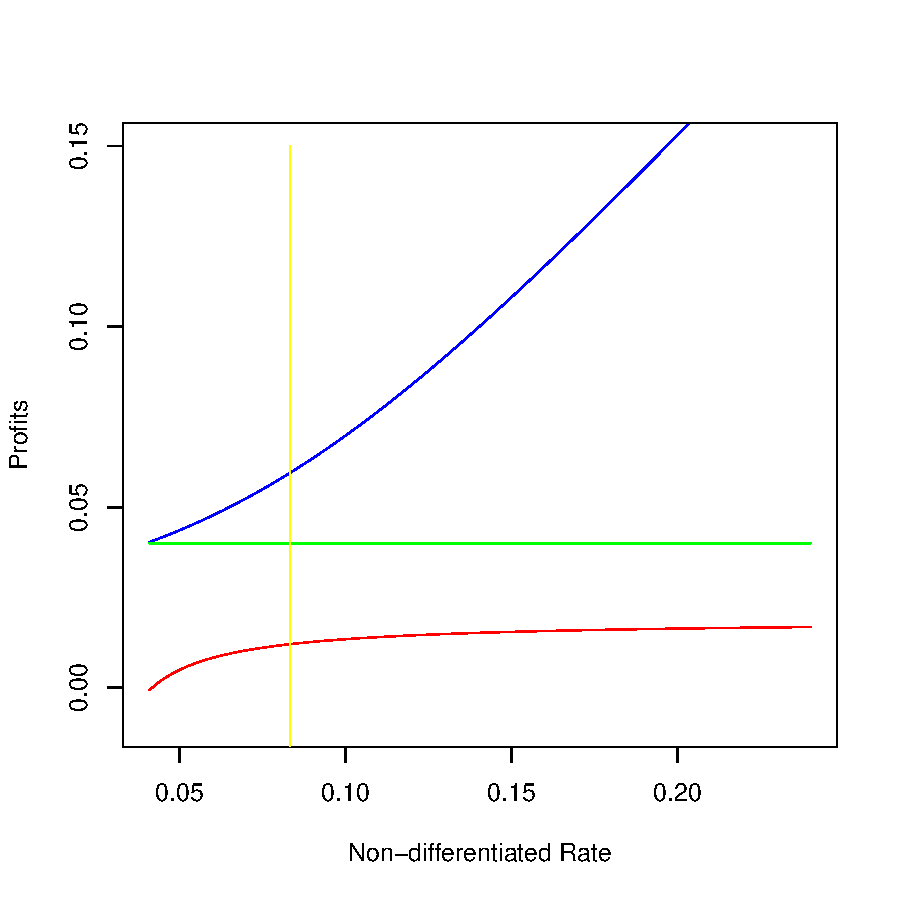
\includegraphics[width=0.5\linewidth]{LoanPricing-fig1plot}

  
  \caption{Profit for each firm for varying rates}
\end{subfigure}%
\begin{subfigure}{.5\textwidth}
  \centering
  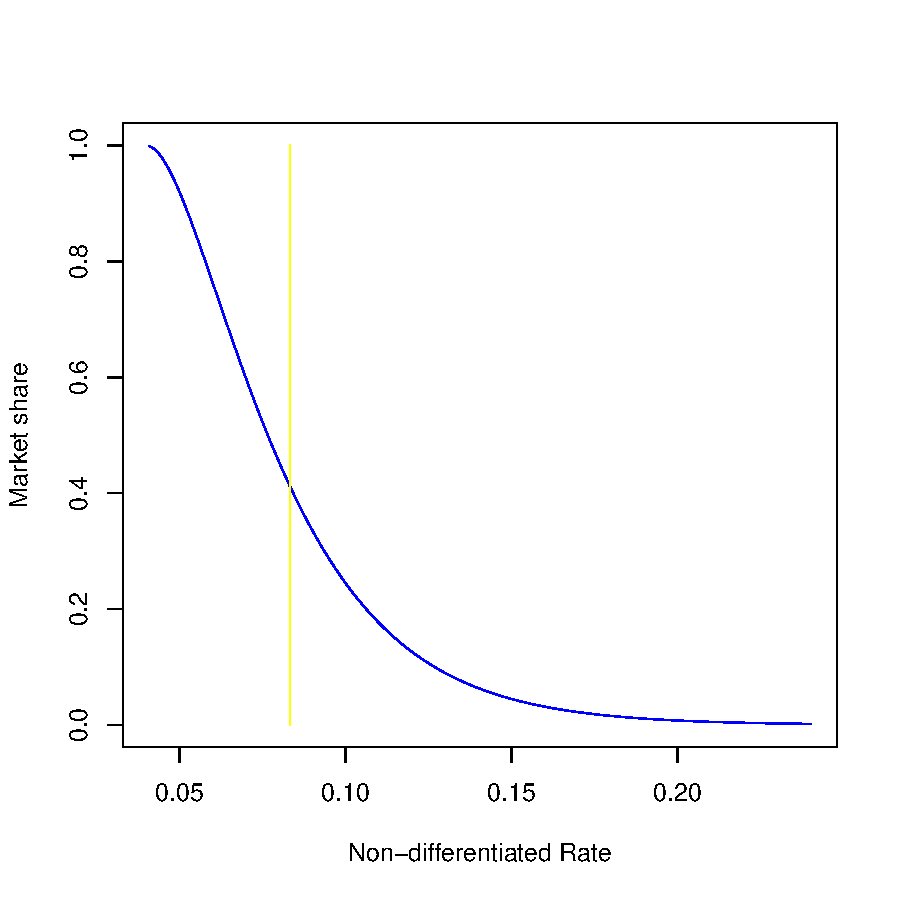
\includegraphics[width=0.5\linewidth]{LoanPricing-fig2plot}
  \caption{Market share for non-differentiated firm}
\end{subfigure}
\end{figure}

As expected, the differentiator dominates the market.  The only hope for the non-differentiator is to charge an extremely high price and try to get the very worst of the loans.  Of course, the non-differentiator is still not profitable and has essentially no market share even in the best case scenario.  
\\
\\
The message to this toy example is clear: better differentation of customers can strongly improve a firm's position in the market.  

\subsection{One firm differentiates and has higher capital costs}

A more interesting scenario is where one where the differentiating firm faces higher capital costs than the non-differentiating firm.  This is similar to a market where a Fintech may have better modeling and additional sources of data for originating loans than traditional retail banks, but has higher capital costs due to the youth of the business and the lack of diversification of its assets.  

In the charts below, \(\alpha=2\), \(\beta=48\), required return for capital for the differentiatior is 8\%, and the required return for capital of the non-differentiatior is 4\%.  


\includegraphics{LoanPricing-004}

\includegraphics{LoanPricing-005}

Now both firms are profitable.  Excess profits for each firm are shown below:

\includegraphics{LoanPricing-006}





\end{document}
